\documentclass[14pt,a4paper]{article}

\usepackage{soul} %пэкэдж для андерлайна
\usepackage{parskip} 
\usepackage{graphicx} %пэкэдж для того чтобы вставлять картинки
\usepackage{amsmath}
\usepackage{hyperref}
\usepackage{enumitem}
\usepackage{geometry}
\usepackage{fancyhdr}
\usepackage{float} %пэкэдж чтобы картинки были на месте
\usepackage{sectsty}
\usepackage[T1]{fontenc}
\usepackage{titlesec}
\sectionfont{\centering\MakeUppercase}

\setul{0.4ex}{0.05ex} % Первая часть регулирует расстояние до текста, вторая часть регулирует толщину линии (для подчеркивания)
% я решила подчеркивания не использовать так как уже болд делаю

\geometry{top=2.54cm, bottom=2.54cm, left=1.91cm, right=1.91cm}

\title{Historical Context of the War in Sudan}
\author{Sezim \& Meirzhan\\
        Nazarbayev University\\}
\date{}

\begin{document}
%\fontsize{14}{14.4}\selectfont
%это для фонта

\maketitle
\tableofcontents
\newpage


\section{Sudan under British \& Egyptian Rule}
\subsection{Sudan’s Geography and its influence on Sudan’s history}
In order to understand the nature of the Sudanese conflict, we first must have a look at its history from the 19th century, its geography, and the circumstances under which the history of the Sudan was shaped. 

\begin{figure}[H]
  \centering
  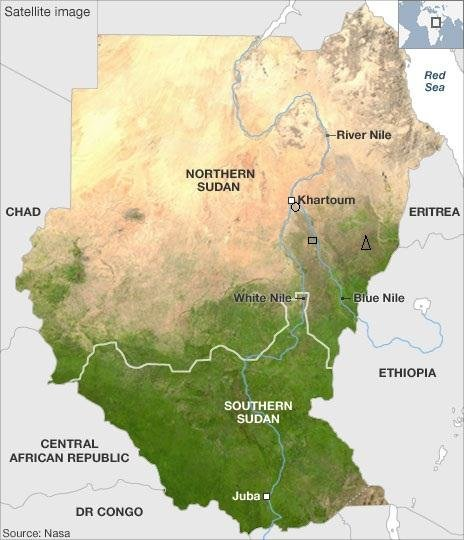
\includegraphics[width=10cm]{figures/sudanmap.jpeg}
  \caption{Sudan map. Source: \href{https://www.mapsland.com/africa/sudan/large-detailed-satellite-map-of-sudan}{Mapsland}} %href для гиперссылки
  \label{fig:label}
\end{figure}


Sudan is located right at the place where the Arab civilization and the native African civilization are intersecting with each other. While the section of the ‘Islamic world’ occupies Sudan’s northern part, the Southern part belongs to the ‘Native African’ culture. 

It comes to no surprise that the divide between two civilizations strongly matches the border between Sudan and South Sudan. \textbf{ Moreover, we can see that Islamic part of Sudan ends exactly at the edge of the Sahara desert while Afro-Christian section occupies the tropical savannah (the green area in Figure 1).} Let’s see how strongly this geographical divide matches the cultural divide of the Sudan: The correlation is very strong.

\begin{figure}[H] %H означает here, можно менять b(bottom), t(top)
  \centering
  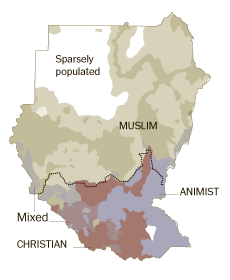
\includegraphics[width=10cm]{figures/religion.png}
  \caption{Religion in Sudan, Source: \href{https://archive.nytimes.com/www.nytimes.com/interactive/2011/01/16/world/africa/sudan-graphic.html?ref=africa}{The New York Times}}
  \label{fig:label}
\end{figure}



\subsection{British governance over Sudan}
The divide that was already pre-determined by Sudan’s geography has been dramatically amplified under the British rule over Sudan between 1899 - 1956. 

During the colonial period, British governors introduced the ‘Southern Policy’ that increased the divide between two parts. As a result of this policy, the northern part of Sudan was going through a rapid industrialization and education while the Southern part remained an undeveloped agrarian counterpart with a mostly uneducated population. \cite{lin2018role} In the end, when Sudan gained its independence, the country was divided not only geographically, ethnically and religiously, but now there was a huge gap in education and economic development. 
British governors never intended for Sudan to remain a single state and they never considered it as one, that’s why the conflict between these two opposite sides was predetermined long before it even began. 


\subsection{Final years of British rule}
By the time the British left Sudan in 1956, they ensured  that the northern (Islamic) elites had gained an overwhelming influence in the Sudanese society and government. They made so through the means of education and economic policies\cite{lin2018role}.  

In 1953, after the first governmental elections were held in Sudan,  the two main parties emerged - Democratic Unionist Party (51 seats out of 97)  and National Umma party (22 seats out of 97)\cite{sternberger1978wahl}. \textbf{Even though these parties had different policies in mind, still they were concerned about the interests of Sudan with the north being its dominant part.} Meanwhile the Southern party obtained only 9 seats out of 97 which left the population of the south out of the political processes of the country in its pivotal historical moments\cite{sternberger1978wahl}. And so Ismail \textbf{al-Azhari} emerged as the first leader (Prime-Minister) of Sudan. 

After the election, the Southern party (renamed as Liberal party of Sudan) was trying to resist the heavy influence of the north-dominated government as much as it could. In 1954, the Southern Party held a conference where it discussed the possibility of the south joining the northern Sudan under the principles of federalism. However, the demands of the Liberal party were ignored\cite{ruay1994politics}.

Later, in June 1955, Liberal Party called for another conference to be held so that they could discuss the unification of all parties of southern Sudan to form a united bloc. However, the north has gained the advantage of the south's disunity and successfully weakened its position as a political force\cite{ruay1994politics}. 


\section{Independence and First Civil War}
\subsection{Beginning of Civil War}
What probably ignited the start of the devastating war were two events: in summer 1955, the southern member of the national assembly was put to trial and there was an alleged telegram from al-Azahri ordering the disarmament of the Southern military regiments\cite{o1977secret}. This, of course, caused a mass discontent among Southerners and so in 1955, on August 18, members of the Equatoria Corps - one of the few military regiments that were loyal to the southern cause - mutinied in the Torit, Equatoria. The mutiny spread across Juba, Yei and Maridi. \textbf{And so began the First Sudanese Civil war.}

\begin{figure}[H]
  \centering
  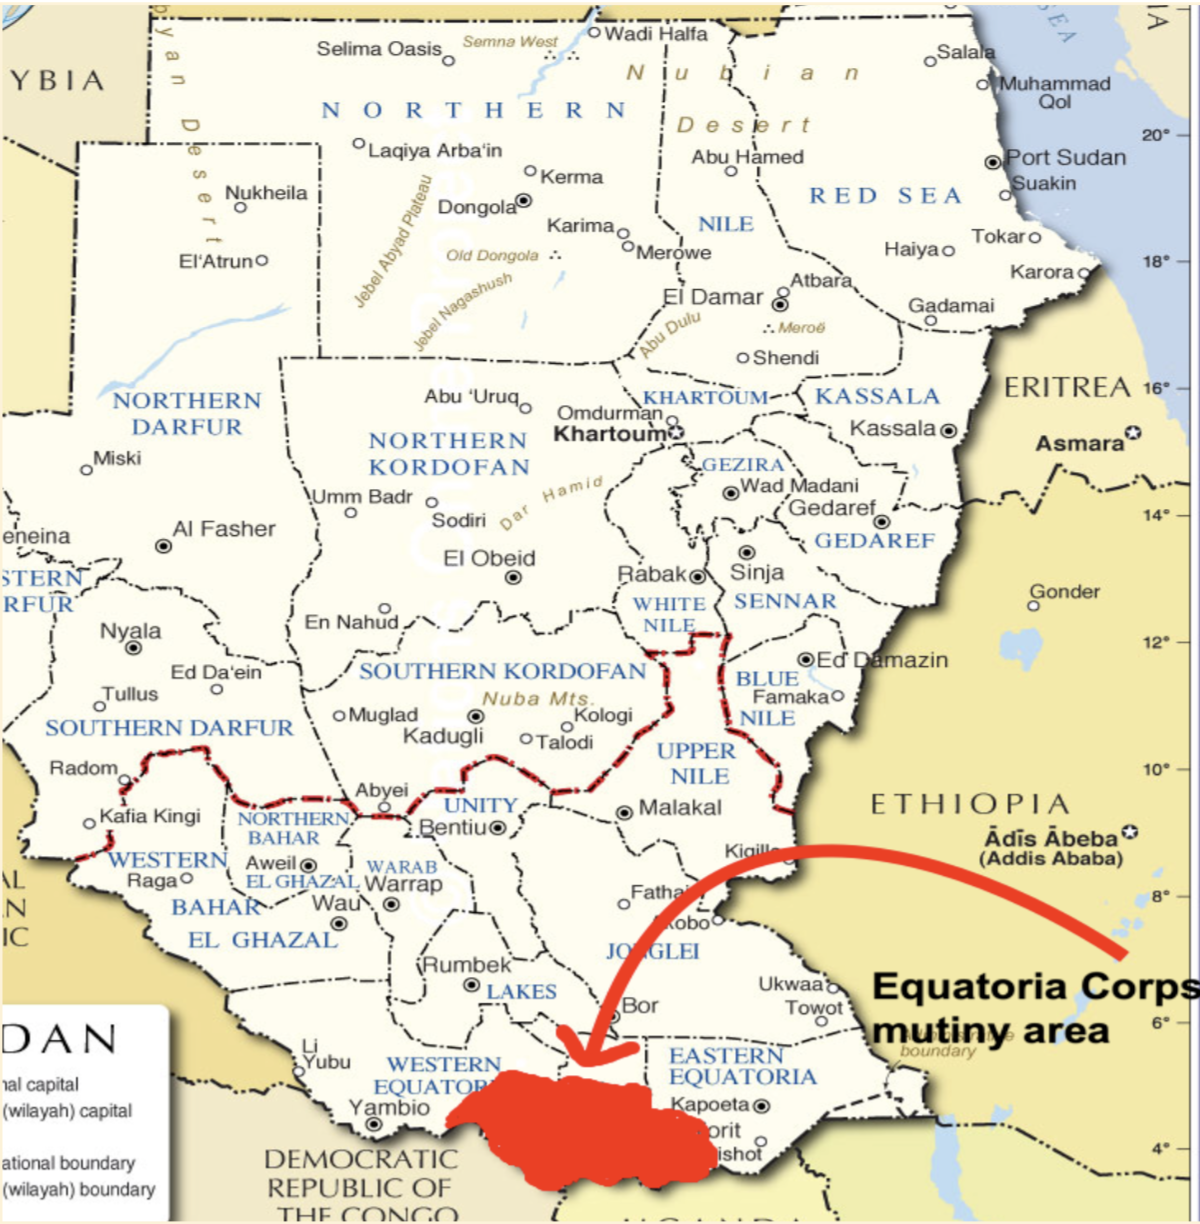
\includegraphics[width=10cm]{figures/EC_Mutiny.png}
  \caption{Equatoria corps mutiny area  (based on information from \cite{o1977secret} )\href{https://www.nationsonline.org/oneworld/map/sudan-administrative-map.htm.}{Nations Online}}
  \label{fig:label}
\end{figure}

In August, 1955  the Equatoria corps mutiny was suppressed by the northern forces and the armed mutineers went to guerilla warfare to neighboring countries. By October 1955, the police and military forces of the south were almost entirely replaced by the northern military units. So began the chain of repressions, starting from sack of villages, confiscation of property, mass arrests ending with instances of unjust executions, tortures and crops burning. Such harsh response to the Equatoria Corps mutiny have significantly widened the  divide between North and South even more.

Tens of thousands of southeners have fled  to the neighbouring countries to avoid the wrath of the Northern militias, soon these refugees will actively support armies of the south\cite{poggo2008first}. \textbf{However, despite the formal beginning of war, the period between 1955 and 1963 could be described as small-scale guerilla warfare rather than all-out civil war\cite{o1977secret}. That’s why the situation in Sudan was still relatively stable.}

On January 1st, 1956, Sudan declared its independence. In 1957, when the Constituent Assembly  was formed, all southern members of the Constituent Assembly withdrew, because the demands for creating a federal form of government were ignored; it meant that southern Sudan had no legal right for self-governance. That, in turn, could have been the reason for further political escalation between Sudan’s Northern and Southern counterparts. 


\subsection{1958 government election and General Abboud's military takeover}
\textbf{1958 saw two pivotal events - the new governmental election and military takeover of General Abboud.} The results of the second governmental election have shown a huge improvement in terms of representation of the Southerns parties. This time they obtained 38 seats (out of 173) in the House of Representatives and 7 seats (out of 30) in the Senate. The Umma party has become the leading party, getting 63 seats (out of 173). However they had to form a coalition with the People's Democratic Party to obtain a majority in the elections. So a new prime minister - \textbf{Abdullah Khalil} - was now in charge of Sudan. 

Under the administration of Abdullah Khalil, from September to November, Sudan was experiencing a sharp economic decline. In October, when the economy of the country was on the verge of collapse, demonstrations broke out in Khartoum. Moreover, because the Umma party was in coalition with PDP, the government was very fragmented. 

On top of that, the army \textbf{general Ibrahim Abboud} announced that “the army would not stand by and watch the country collapse”. This statement was rather surprising to the Sudanese population because for them, the army wasn’t associated with politics too much. 

Realizing his doomed position, Abdullah Khalil decided to voluntarily give up the power in the hands of the military. So, on November 17, 1958, \textbf{general Abboud} took charge of the country in a bloodless coup. The coup was welcomed by the Northern Sudanese, because they were seeking political and economic stability. There was a belief among northerners that the “army would put an end to the southern problem with an iron first”\cite{poggo2008first}.

\subsection{General Abboud's rule}
The ruling style of Abboud's military administration was indeed an 'iron fist'. It was accompanied by the harsh military policing in the regions of Bahar El-Ghazal, Equatoria and Upper Nile. 
The reason for that was to prevent local population from collaborating with the Southern rebels, who were waging a guerilla warfare from the border regions of neighbouring countries. \cite{poggo2008first} 

\textbf{Moreover, one of the key policies that defined General Abboud's rule was forced Islamization and Arabization of the Southern Sudan}. Accroding to \cite{poggo2008first}, "Its primary objective was to undermine Southern traditional laws and customs in maintaining justice, law and order, and harmony among the various ethnic groups. Abboud’s administration wanted to replace African laws with Islamic laws as part of its program of Islamization in the South."
To achieve this goal, General Abboud used both military force and civic measures.

When it comes to military force, General Abboud have established a very harsh martial law in the southern provinces. Moreover, the mass persecution, torture and murders have now began in the region, especially in those areas where locals were suspected of helping guerilla soldiers.
The northern military units have become the majority of armed forces in the Southern Sudan, because southern army have come under a huge distrust from the newly established administration in Kharotum. At this point, northern troops resembled an army of occupation rather than security force and they acted accordingly.
The presence of Northern military was marked by constant atrocities and violation of basic rights such as presumption of innocence - everybody, whether they were guilty or not, have become the possible victims of harsh repressions\cite{poggo2008first}

\begin{figure}[H]
  \centering
  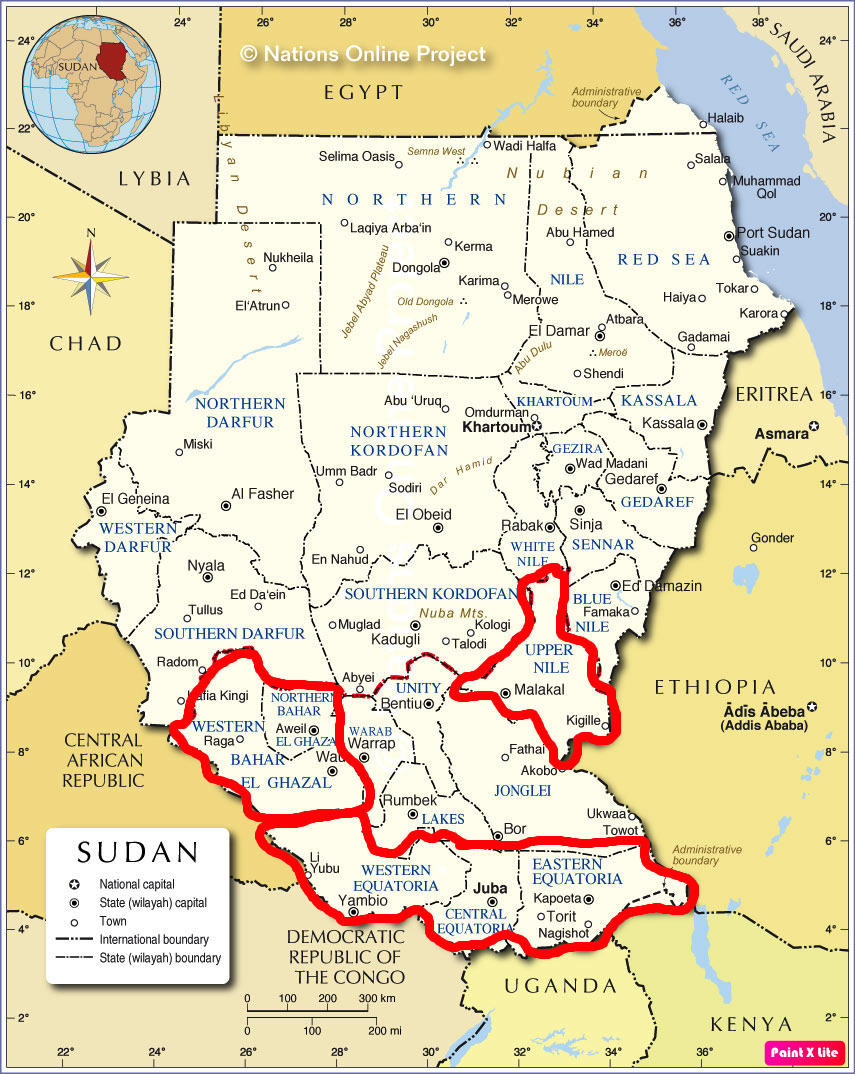
\includegraphics[width=10cm]{figures/HarshRepressionsMap.jpg}
  \caption{Area of most intense repressions (based on information from
  \cite{poggo2008first} )\href{https://www.nationsonline.org/oneworld/map/sudan-administrative-map.htm}{Nations Online}}
  \label{fig:label}
\end{figure}

Some disturbing changes were seen in the administrative, educational and religious spheres.
First, the chiefs of the southern province were forced to accept Islam under the threat of losing their positions. In addition, the government in Khartoum have put a huge emphasis on publicly announcing the names of those who have converted to Islam so that Southern population was led to belief that Islam quickly spreads through their governors and that it's time for them to do the same
Second, Arabic language and teaching of Islam was widely introduced in the Southern academic institutions. As \cite{poggo2008first} points out "In 1960 through 1961, knowledge of Islam and the Arabic language became a requirement for admission to Southern schools" (p. 95). Moreover, Arabic was now becoming a language of instruction in all southern schools so that local population could better connect with the Arabic culture and eventually embrace the Islamic values. 
Third, the policies towards Christian institutions in the South were becoming more and more strict. The official policy of Abboud's administration suggested that the Christianity must be replaced with Islam to make Sudan a unified nation. In \cite{poggo2008first}, a local government official in Upper Nile province argued that "Our main aim is to see that you call yourselves Muslims...Christianity is a foreign religion and should have returned to Europe with the colonialists" (p. 94)

General Abboud's 'iron fist' methods, despite that they were welcomed in 1958-1959, have led to the growing unrest among civil population both in Northern Sudan and especially Southern Sudan. 
In attempt to fix things up, Abboud have established a commission that was supposed to thoroughly study the situation in a country and make recommendations for the solution of the problem.
Because this commission have began an open debate about a 'southern problem' the Sudanese students have begun actively participating in it and soon these debates have turned into a forums for open critiscism of the government's actions. Such activities were then forcefully suppressed by the government but it started the chain reaction that have led to the mass protests across the country \cite{Berridge2014October}.
Abboud had to yield to the demands of the protesters and he dissolved his government (The Supreme Council) on October 26, 1964 and a new prime minister took charge of the country -  \textbf{Sirr Al-Khatim Al-Khalifa}. 

\subsection{The South strikes back}

\subsubsection{Resistance consolidates}

As it was noted before, in the first 8 years of Civil War, southerns resistance was resembling more of a banditry acts in the countryside rather than properly coordinated guerilla warfare \cite{o1977secret}. All this time, the resistance movement was fueled with more and more people who were fleeing from the Southern regions to avoid persecutions.

The intensive repressions conducted by the General Abboud's administration haven't been unnoticed. The main consequence of Supreme Council's (so was called general Abboud's government) policy was thousands of Southeners fleeing to neighbouring countries - Central African Republic, Uganda, Congo and Ethiopia. Among these refugees were not only women and children, but also southern politicians, ex-military men and southern students \cite{poggo2008first}. 

In 1962 the key moment of South's consolidation occurred: the formation of Sudan African Closed Districts National Union (SACDNU),the first southern opposition party in exile. It's main leaders were William Deng, Father Saturino, and Joseph Oduho \cite{rolandsen2011making}. Later, in 1963, the party was renamed to Sudan African National Union (SANU). SANU focused on gaining international recognition, political and economic support of foreign countries and raising a proper army to challenge the rule of Sudan's government \cite{rolandsen2011making}

In August 1963, southern politicians and military leaders met in Kampala, Uganda to discuss the 'formalization' of the armed resistance movement, its strategy and military plans \cite{poggo2008first}. They chose the name of Anyanya that translates as "Snake Venom" in Mahdi language. 

\subsubsection{Anyanya attacks}

Anynya have launched its first military offensive in September 1963 in Eastern Equatoria. \cite{poggo2008first} (p. 68). Soon, the attacks were noticed in Central Equatoria as well, where resistance was led by Father Saturnino and Joseph Lagu (A sudanese commander who decided to turn from Kharotum administration and join the southern resistance) \cite{rolandsen2011making}, p. 224. 

The element of surprise was sure an advantage of the Anyanya attacks, but soon they were not effective anymore, because Sudanese military and police were now on their guard, so the Anyanya attacks were becoming less and less efficient. In addition, the rebels were poorly armed; they had to fight with bows, spears and Molotov cocktails while the majority of armed rifles they had were war trophies taken from the Sudanese soldiers \cite{rolandsen2011making}. 

\subsubsection{Southern Sudan provisional government forms}

Despite that Anynya forces were ill equipped and heavily relied on the support of local population and foreign aid, their military efforts against Sudanese army were not unnoticed. Moreover, all this time from 1963 to 1967, the political movement of the Southern resistance was slowly but gradually developing and in 1967 saw two major events - the death of Father Saturnino (the founder of Anynya) and emergence of Southern Sudan Provisional Government (SSPG).
A politican Aggrey Jaden was elected as a president of SSPG.

\subsubsection{Anyanya is reformed and getting stronger}

Under the administration of Aggrey Jaden a huge efforts began to turn Anyanya from decentralized resistance movement where each resisting tribe was operating in its own region to a centralized army with a centralized command \cite{poggo2008first}. So he renamed Anyanya to Anya-nya Nation Armed Forces (ANAF) to highlight the national mission behind the army's actions \cite{poggo2008first}. 

\subsubsection {A minor setback and change of tactics by Joseph Lagu}

Because Anya-nya still wasn't totally centralized and its commanders in 3 different regions - Equatoria, Upper Nile and Bahr al-Ghazal had quite different views regarding the future of the movement, it has led to a series of scirmishes within the movement and they [commanders] were partly interested in keeping that internal division to not lose their power to each other. \cite{poggo2008first}
In the heat of the skirmishes, commander Joseph Lagu - who founded Anya-nya together with Father Saturnino and commanded the same amount of respect and authority among southern elites - emerged as a military leader of the ANAF. He opposed the idea of centralized Anya-nya command and instead insisted that each local group should operate in its indigenous region because that would be the most efficient strategy to properly resist Sudanese troops. However he made sure that all factions of the Anya-nya resistance would keep in touch with him and recognize him as a central figure of the ANAF. 

\subsection{Time of political disaster in the North and general Nemeiry's takeover}

While Anya-Nya movement was consolidating, gaining more power, local and foreign recognition, the situation wasn't that good for the Kharotum government. 
After General Abboud's Supreme Council's fall, sir Al-Khatim Al-Khalifa took his place. Because Al-Khalifa couldn't solve the Southern problem and was sympathetic to the Sudanese communists, he didn't enjoy too much popularity even though he tried to introduce numerous reforms in the country.
He was replaced on the next year in 1965 by Muhammad Ahmad al-Mahgub - a member of the National Umma Party. On the next year, in 1966, al-Mahgub was replaced by yet another prime minister - Sadiq al-Mahdi, who was also a member of the Umma Party and emerged as its new leader after factional division. 
What's more interesting is that Sadiq al-Mahdi lasted less than a year and was again replaced in 1967 by the previous prime-minister al-Maghub who now claimed the leadership over the Umma Party. 

All this time though, the position of 'head of the state' from 1965 to 1969 belonged to the Ismail al-Azhari, the first elected Prime Minister of Sudan in 1953. 

Dissatisfied with such constant change of power, another military takeover happened in 1969. This time around, it was conducted by the military general Gaafar Muhammad an-Nimeiry. It was he who arranged the peace agreement with the South Sudan Liberation Front in 1972 (SSLF) and put an end to the war that lasted for almost 20 years. Because of that move that has put an end to the bloodshed that has lasted for two decades, Nimeiry have enjoyed a good reputation both inside the Sudan and outside out of it \cite{kasfir1977southern}

\subsection{Peace negotiations and Addis Ababa Agreement}

In 1972, in the face of South's resistance consolidation and deep political crisis in the Sudanese government in Kharotum, a treaty was signed in Addis Ababa and was observed by Ethiopian Emperor Haile Selassie with General Nemeiry representing the Sudan and Joseph Lagu (a resistance leader) representing the Southern Sudan. 
This treaty paved a way for a huge reforms and establishment of various agreements with the South that addressed South's desire to obtain the autonomous status within a unified Sudanese state. It eventually marked the end of the First Sudanese Civil War and Sudan's, although short-lived, reconciliation. 


\section{Second civil war}

\subsection{Addis Ababa Agreement and aftermath}

Based on the Addis Ababa Agreement signed in 1972, three main concerns of the Southern side were addressed:
\begin{itemize}
        \item Create a separate government of Southern Sudan with its own legislature and executive body. Granting autonomy for Southern Sudan. 
        \item Integration of the Anya-nya rebels into the military and police forces
        \item Unification of South Sudan within a Sudan state and end of the South's division into three separate regions - Bahr al-Ghazal, Equatoria and Upper Nile
\end{itemize}

\subsection{Change of Nimeiry's political course and violation of agreement}

Initially, general Nimeiry was known for not being influenced by the Islamic agenda of the Northern elites. That is the reason why he wasn't so resistant to give such concessions to the Christian-Anemist south.

However, in the mid 1970's, the rise of support of militant groups like "Ansar" movement and "National Islamic Front" coupled with rising support of Darfurian soldiers (who are strongly associated with Islam) made general Nimeiry to conduct a policy of appeasement of these groups to not lose his power. 

In addition, the discovery of oil reserves along the North-South border led to the decision of Nimiery's administration to push the border between two counterparts further south, because Kharotum government wanted to obtain as much resources as it could, ignoring the fact that such decisions were violating Addis Ababa agreement. \cite{raftopoulos2006peace} pp. 12-13

So, in 1983, he declared Sudan an Islamic state and abolished the Southern Sudan autonomous region, which of course, was a direct violation of the Addis Ababa agreement. \cite{derouen2007civil} p. 745


\subsection{Beginning of war}

The radical turn to Islamism by general Nimeiry (who probably did it under the pressure of different Islamic elites) and his bold decision to march against Addis Ababa agreement in 1983 have sparked the wave of mutinies in the Southern Sudan cities. Nimeiry have sent in the army to suppress the mutiny, but the army was repelled by the mutineer forces \cite{johnson2003root} p. 209. And so began the second civil war which was a continuation of the North-South struggle. 

\subsection{Sudan's People Liberation Army emerges}

In response to such harsh reaction by the central government, the Sudan's People Liberation Army emerged as rebel group in 1983 led by John Garang. Important to note, that this movement, unlike its predecessors from First Civil War, did not intend to advocate for South's interests only but rather unite ALL people who were dissatisfied with central government of Nimeiry. It aimed to obtain power over the entire Sudan and create a new government based on the values of diversity - to bring idea of "New Sudan" into reality. \cite{raftopoulos2006peace} p. 13. 

However, the Sudan's People Liberation Army (SPLA) shouldn't be perceived as a movement that has successfully united the whole south, because it had a reputation being a Dinka militia \footnote{Dinka was a dominant tribe in the South and all other tribes perceived the formation of SPLA as an attempt of Dinka to gain power over the country}. That's why many other tribe preferred to form their own resistance units instead of joining a united SPLA army. 

\subsection{Military coup of 1985 and 1986 elections}

\subsubsection{Military coup in 1985, revoking few Islamist decree's}

Because the civil war led to the economic decline of the country and to the worsening relations with the United States, a protests broke out in Kharotum in 1985. Dissatisfied with such chaotic situation, military launched a coup against Nimeiry.
The new government revoked the decree issued by Nimeiry's government - a decree that highlighted Sudan's course to becoming an Islamic state. 

\subsubsection{Negotiation with SPLA, trying to end civil war}

Despite that the newly established government in Kharotum aimed to end the civil war, SPLA wasn't so eager to negotiate with them. Mostly because there were still a lot people who remained in their seats after Nimeiry's replacement and because that majority of northern population and elites still supported the enforcement of Sharia law across the entire country.

\subsubsection{Election of 1986}

As was promised by the military council that came to power after overthrowing general Nimeiry, they held an election and gave up the power to civilian administration. 

As a result of the 1986 election, a leading party coalition emerged that consisted of Umma Party, National Islamic Front (NIF) and the Democratic Unionist Party (DUP). Sadiq al-Mahdi - a member of the Umma Party - was chosen a prime minister and he heavily advocated for the implementation of Sharia law.

\subsubsection{Second negotiation with SPLA}

In 1988, DUP conducted a series of negotiations with John Garang (leader of SPLA) and they came up with a plan of peace proposition that included putting Sharia law to a halt, a call for ceasefire and end of state of emergency in Sudan. However Sadiq al-Mahdi, being a very strict follower of Islamization politics, have rejected the plan. In response to that, DUP left the government in 1988. But in the following year, after series of victories of the SPLA in the south and capture of few important cities, the army forces would pressure al-Mahdi to approve this peace proposition and form a new government with DUP, otherwise army threatened to forcefully replace him. Al-Mahdi submitted to demands, but NIF have left the government as a sign of protest: soon NIF will mike its first bold move together with colonel Omar al-Bashir \cite{johnson2003root}. 

\subsection{Revolutionary Council and Omar al-Bashir's takeover}

In Jun 30, 1989, Omar al-Bashir and his Revolutionary Command Council for National Salvation (RCC-NS) have overthrown Sadiq al-Mahdi's government and established a military junta consisting of 15 military officers. NIF was allegedly involved in this affair \cite{globalsecurity}, because Omar al-Bashir was a suitable person to fulfill NIF's wish to crush the South and introduce Sharia law across the Sudan. In addition, the leader of NIF - Hassan al-Turabi - was now enjoying some degree of religious and political power. It's under al-Turabi's watch Sudan was hosting a various radical Islamists group from across the globe; Sudan hosted Osama bin-Laden for some time in Kharotum where he was provided his own residence facility. 

In response to al-Bashir's takeover, SPLA (South), DUP (North), Umma party (North) and some minor tribal and political groups have decided to create a party coalition - National Democratic Alliance (NDA) - to oppose al-Bashir's regime. 

In 1991, al-Bashir's government issues a 1991 Criminal Act where various brtual Islamic laws were introducted across the entire country, including such crime punishments as stoning and amputations. In addition, a 1991 Public Act was introduced where mixed gatherings of men and women were prohibited. The non-Muslim judges in the South were gradually replaced with Muslim ones.

\subsubsection{SPLA divides and al-Bashir attacks}

One particular group within, which was made of Nuer tribe militias, were pursuing the goals of South Sudan's liberation as well, however they were deeply dissatisfied with SPLA's leader - John Garang. So they planned to overthrow him and even made few unofficial agreements with Kharotum's regime about it. After a failed coup attempt due to lack of support within SPLA, they've become a completely separate fraction - SPLA Nasir - that positioned itself as hostile to the SPLA, but still fighting for the Southern cause. 

After figuring everything out, John Garang (leader of SPLA) sent in the army to the Upper Nile region (controlled by SPLA Nasir) to disarm and neutralize this faction. However the attack was repelled. 

In 1992, Sudanese army exploited this moment of weakness of the Southern front and delivered a few critical blows to the SPLA. On top of that, Ethiopia stopped supporting Southern factions, because its former leader Mengistu Haile Mariam was toppled and the new government of Ethiopia was leaning more towards al-Bashir's administration rather than John Garang's one. 

Because SPLA Nasir now openly aligned with Kharotum governement and received arms from it, because they were negotiating the status of South as a part of Sudan and because they've let the government army pass through its territory, it heavily damaged their reputation in the South. In the future, it has led to a lot of defections from the Nasir to the John Garang's camp. 

\subsection{South strikes back (again)}

In 1995, a counter-attacked followed by SPLA that have brought vast territories which were taken by Kharotum governemnt in 1992 back to the South's fold \cite{johnson2003root} pp. 100-5.

Moreover, because the government of al-Bashir was strongly associated with supporting Islamic terrorism across the world (thanks to al-Tarabi's and NIF's actions), the sympathies of international community, especially USA government, were leaning more towards South Sudanian cause: this have isolated Sudan government even more. 
Not only that, but because al-Tarabi was supporting the radical Islamic rebels in Eritrea and Ethiopia, these two allies of Sudan have switched sides and decided to support SPLA instead. 

\subsection{The war ends}

For al-Bashir, the priority now was to find any way that can end the Civil War as soon as possible, because Sudan found itself in a very sticky situation where the internal 'Northern' opposition have sided with the Southern rebels, where the Southern rebels are receiving aid and military support from different countries including direct military intervention by Ethiopia and Eritrea (until 1997-1998), where Sudan was now isolated from international politics because its religious authorities, namely al-Tarabi and NIF, have openly cooperated with various Islamic terrorist organisation around the globe (Al-qaeda, Hesbollah, Hamas, Jemaah Islamiyah). So he decided to arrange separate negotiations with different rebel groups. From 1997 and on, the situation on the frontline didn't change that much, because the long process of negotiation with various Southern rebel groups have began, despite that the problem wasn't solved in a day, by the year 2005 a peace agreement was achieved that have officially ended the Second Sudanese Civil War. 











\section{Darfur Conflict} %быля как этот секшн инкорпорейтить, соу фар кажется как отдельный конфликт, нот рилейтед??? :с
\subsection{Preconditions for the conflict in Darfur}
Disputes in the area are recorded back from 1939 and generally arise from the access to natural resources. In February 2003, two armed groups waged war against the Government of Sudan. Sudan Liberation Army (SLA) and the Justice and Equality Movement (JEM). Many have fled to neighboring Chad. Sudan has welcomed, hosted and facilitated a wide range of missions and delegations from western countries, and international and regional organizations. These have included visits from British Prime Minister Tony Blair, the United States Secretary of State, Mr. Colin Powell and Ministers from, amongst other countries, Britain, Germany, France, Spain, Switzerland, Italy, Ireland and Canada.

Most of the victims are Arab pastoralists from tribes that backed the government's fight against the insurgents. They were promised loot, land, and sometimes salaries after years of being ignored, during which their rights to pasture and water were taken away and they were deprived of basic services.
The conflict escalated again in 2010, turning into intense battles between camel-herding Abbala and cattle-herding Baggara tribes. Specifically, it involved parts of the Northern Rizeigat Abbala and various Baggara tribes allied with the Missiriya. Both sides freely use weapons provided by the government. %засайтить
%is it even relevant?? :c
\subsection{How the war went, general timeline}
\textbf{February 2003} – Two anti-government groups rise up, saying Khartoum neglects arid regions and arms Arab militia against civilians.

\textbf{January 2004} – The army moves to quell the uprising in western region of Darfur; hundreds of thousands of refugees flee to neighboring Chad.

\textbf{March 2004} – UN says pro-government Janjawid militias are carrying out systematic killings of African villagers in Darfur.

\textbf{April 2004} – Government, Sudan Liberation Army (SLA) and Justice and Equality Movement (Jem) fighters agree on ceasefire.

\textbf{September 2004} – UN says Sudan had not met targets for disarming pro-government militias and must accept outside help to protect civilians. Colin Powell, US secretary of state, describes Darfur killings as genocide.

\textbf{May 2006} – Khartoum government and the main anti-government faction in Darfur, the Sudan Liberation Movement, sign a peace accord. Rival SLA faction and the smaller Jem reject the deal.

\textbf{August 2006} – Sudan rejects UN Resolution 1706 calling for a UN peacekeeping force in Darfur, saying it would compromise Sudanese sovereignty.

\textbf{December 2006} – Sudan agrees in principle to accept the deployment of UN troops in Darfur as part of an expanded peacekeeping force.

\textbf{February 2007} – International Criminal Court’s chief prosecutor names first two war crimes suspects in Darfur. Sudan says the ICC has no jurisdiction and rejects arrest warrants.

\textbf{May 2007} – George Bush, US president, imposes new US sanctions on Sudan and asks for support for an international arms embargo to end what he calls genocide in Darfur.

\textbf{October 2007} – Darfur peace talks open in Libya and the government declares an immediate unilateral ceasefire, but important anti-government groups are absent.

\textbf{May 2008} – Jem fighters make a lightning attack that reaches the outskirts of Khartoum. About 65 people were killed.

\textbf{October 2008} – Al-Bashir pledges more co-operation with Unamid to secure the passage of aid convoys, along with up to \$350m of spending on development in the region. The UN says up to 300,000 people have died in Darfur and some 2.5 million have fled their homes since 2003.

\textbf{February 2009} – Sudanese army declares the capture of a town in Darfur after three weeks of clashes with Jem fighters. Qatar hosts first peace talks in nearly two years between the Sudanese government and Jem rebels with the two sides agreeing to undertake “good faith” measures.
February 2010 – Appeals chamber of the ICC directs judges to rethink their decision to omit genocide from the warrant out for al-Bashir’s arrest. Idriss Deby, Chad’s president, makes a landmark trip to Khartoum. He and al-Bashir announce their intention to normalize ties. Later Jem announces an accord with Sudan’s government leading to a ceasefire, to be signed in Qatar \cite{AlJazeera}.


\subsection{Darfur deal}
Several peace agreements were attempted, but lasting peace proved elusive. The most notable attempt was the Darfur Peace Agreement signed in 2006, which failed to end the violence.

\section{South Sudan Independence}
\subsection{The Comprehensive Peace Agreement (CPA) \& Conversation around independence}
The fight over oil has contributed to the collapse of the Addis Ababa agreement mentioned earlier in this document. However, the political exclusion is what made southerners rebel for nearly two decades and active Arabization of the Sudanese peripheries provoked a rebellion in Darfur in 2003 and sparked the tensions in Southern Kordofan and the eastern part of the state \cite{challenges}. 

The CPA has been a major step towards ending the bloodbath that has been going on for decades and it was signed in January 2005. It was composed of the Machakos Protocol, the Agreement on Wealth Sharing, the Protocol on Power Sharing, the Protocol on the Resolution of Conflict in Southern Kordofan and the Blue Nile States, and the Protocol on the Resolution of Conflict in the Abyei Area. The civil war ended when SPLA and the government of Sudan signed the CPA on January 9, 2005. Both parties attempted to popularize the narrative of a unified Sudan ('New Sudan', supported by Garang) through the agreement to make everyone equal in the country after the Civil War ended. 

During the peace negotiations involving the US, it was proposed to replace the Islamist regime with 'New Sudan', a state run by SPLM. In the Machakos Protocol, parties prioritized unification while keeping the independence of Sudan as an option. If unification under 'New Sudan' would be impossible, then the final solution would be total independence of Sudan so it has opened a door for the future split of South Sudan. The protocol required the involvement of member states of the IGAD Sub-Comittee on Sudan, observer states (Italy, Norway, UK, and US) and any other countries or international bodies to be agreed upon by the parties.

As the National Congress Party (NCP) and SPLM failed to create the unified state of Sudan as they failed to represent the interests of southerners, they began to consider the possibility of independence \cite{NewSudan}. Especially, after Garang's death, SPLM lost its most active supporter of the idea of unified Sudan. As a result, SPLM withdrew from active participation in national politics which resulted in a more centralized government led by NCP. 

Though the CPA has been successful in achieving peace for some time, it has never achieved its aim - the unification of Sudan. Conversely, after the SPLM withdrawal from political participation, Sudanese people would be voting for the independence of South Sudan. 



\subsection{Issues delaying the independence of South Sudan}
However, there were multiple challenges to achieving this objective. Firstly, sharing the country's oil wealth was an issue since oil reserves were mainly located in the south or the north-border region, but the pipelines and the main infrastructure ran through the north. Oil revenue is of major interest to both the north and south. However, this is especially true for South Sudan as it gets most of its revenue from oil. Moreover, the ongoing corruption in the oil industry has made it difficult to create a framework for calculating and sharing oil reserves. The inconsistencies in the reports on oil revenue have raised mistrust between the states and made it difficult for them to cooperate. So a coalition of governments, companies, and civil societies promoting transparency is a vital step towards resolving the issue. 

Apart from the oil issue, sharing the country's collective debt and establishing the borders around the Abyei region has been a big challenge as well. Abyei region is very fertile and its significance in oil production and River Kiir(in Dinka) is high. For this reason, the final demarcation of this region has raised tensions between the North and the South. This dispute caused multiple clashes involving NCP, the Misseriya, and SPLM that made the locals flee the region and led to dozens of deaths. After these clashes, the CPA has established that Abyei would be a bridge between the North and the South which means that its inhabitants will have citizenship of both Sudanese regions. 

%elaborate on that, the corruption over oil, ethnic conflict within South Sudan and its economic dependency on oil resources. 
%proxy militas in South Sudan.
\begin{figure}[H]
  \centering
  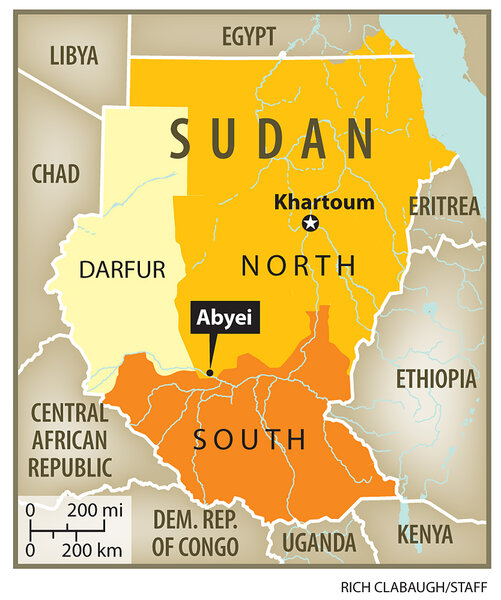
\includegraphics[width=10cm]{figures/OABYEI_g1.jpg}
  \caption{Geography of Abyei region from \href{https://www.csmonitor.com/World/Africa/Africa-Monitor/2010/1102/Oil-rich-Abyei-Time-to-update-the-shorthand-for-Sudan-s-flashpoint-border-town}{The Christian Science Monitor}}
  \label{fig:label}
\end{figure}


%написать про партис инволвд а регион абйей (????) и как эти дела сейчас рашеаются. 

\section{South Sudan after obtaining Independence}
\subsection{Government of South Sudan}
As previously mentioned, Sudanese governance has long been corrupt which means that political office was used for personal advantage of the Sudanese elites. Following the death of J. Garang, ex-SPLM(-A) leader, Kiir has become a president of autonomous Government of South Sudan(GoSS) and later would be a president of South Sudan. His ruling style would be similar to what Sudanese government did. 

South Sudan's political situation was very unstable after the independence because of how they ruled their peripheries and by militarizing tribes in the region. SPLA which fought against Sudanese government ended up adopting a lot of its practices, especially after the CPA was signed. 

Both the North Sudan and South Sudan heavily relied on financial patronage and used the money for the defense. South Sudanese government focused on getting rich faster and ensuring to build a strong army to deter the northern Sudanese government. This led to an increase in SPLA (Sudan People's Liberation Army) size even after the war ended, in response to the north’s increasing defense spending.

In comparison to neighboring countries, which directed government spending towards infrastructure and health services, South Sudan's monetary reserves were either stolen or allocated to the military. Kiir's strategy of over-investment in the armed forces worked before the referendum as we can see that 98.83 percent voted for secession of South Sudan. However, by 2013, the South Sudanese government couldn't afford to keep paying for the loyalty needed to maintain the system, causing it to collapse. \cite{de2014kleptocracy}



\subsection{Another Civil War}

%As it can be observed, Sudanese and Central African countries used to use violence as a form of bargaining. A provincial leader would be using mutiny or a rebellion to claim resources over the region. Agreement would be reached only after dozens of deaths and displacement of local citizens. In South Sudan this is known as "rent-seeking rebellions". %make this relevant
\subsubsection{Escalation}
%здесь написать про диспутс и из-за чего они вообще шатнули производство нефти?
President Kiir fired his cabinet, including Vice President Riek Machar because of the coup d'etat accusations which gave rise to discontent among people.  

Apart from that, following disputes over oil with North Sudan, the South Sudanese government halted oil production for six months. Since oil production accounted for most of the country's revenue, this decision exacerbated South Sudan's already fragile state, paving the way for local mutinies. 

The political crisis quickly escalated into a war. Due to the lack of structure in South Sudan's army, it fragmented into multiple factions based on ethnicity. The issue of ethnic tensions existed decades before the CPA and was overlooked during discussions of self-determination during that time, as southerners were treated as a single group. It may have happened because they fought under the same banner during the struggle for independence. In reality, the region comprised many different ethnic groups. 

Following independence and the state's economic fragility, South Sudan's militias and elites divided along ethnic lines, each vying for control over the region's resources. The conflict primarily involved the Nuer against the Dinka ethnic groups, with the Dinka, the predominant ethnic group in South Sudan, supporting the incumbent president, Salva Kiir, while Nuer supporting its vice-president, Riek Machar, who began to criticize Kiir's policies.

The consequences of the civil war have been significant. According to \cite{rolandsen2015year}, the war have led to the deaths of nearly 100 000 people, including those who died from illness and malnutrition caused by the war. By December of 2014, approximately 2 million of people have been displaced, including those who fled the region. 

The oil production has been reduced by 30\%, and the ongoing war has discouraged the foreign investment which led to a significant economic downgrade. \cite{rolandsen2015year} reports that economic recession gave an advantage to SPLM(A) in peace negotiations, as government is heavily dependent on oil revenue. 

\subsubsection{The war and its violence}
Rebels used radio to broadcast war songs and hate speech towards each other. One of the interviewed women whose children suffered murder said that she supports violence and desires for all of the Dinka people, including children, to be dead. 

\subsubsection{The key players in the Conflict}
\paragraph{Pro-Government forces} \mbox{}\\
Pro-Government forces included security forces of the SPLA, South Sudan National Police Service (SSNPS), wildlife and prisons services, troops from
the Uganda People’s Defense Forces (UPDF), community-based Dinka militias, and Sudan-based
supporters such as the Sudan People’s Liberation Movement-North (SPLM-N), from South Kordofan, and
the Darfuri Justice and Equality Movement (JEM) \cite{observer2014military}. 

%доделать секшн и добавить про кей плэйерс отсюда https://www.enoughproject.org/files/Military_Dynamics_of_South_Sudan_Civil_War_-_Enough_Forum_-_July2014.pdf

%need more elaboration. 
%https://academic.oup.com/afraf/article/113/452/347/78186 дочитать

%Darfur structurize and write abt it to connect to independence
\paragraph{SPLA} \mbox{}\\
The SPLA, now largely Dinka-led, has seen many Nuer troops defect to the opposition. The government lost most of the Upper Nile region early in the conflict and recruited 20,000 new fighters in four months, including children. In January 2014, Central Equatoria Governor Konga called on all forces to defend against rebels, and Vice President Igga aimed to mobilize 5,000 to 10,000 recruits. 

The Central Equatoria security advisor urged ex-combatants and youths to join the army, promising short training and immediate pay. Forced and voluntary recruitment, including of children, happened across South Sudan, leading to untrained recruits on the frontlines and high casualties.

\paragraph{Dinka militias} \mbox{}\\
The government has relied on community-level Dinka militias like the Gelweng, pastoralist youth cattle guards involved in early violence in Juba. Historically, the Gelweng have functioned as Dinka paramilitary forces, aiding and sometimes fighting against the SPLA.

In late 2013, 15,000 Gelweng were allegedly recruited as part of President Kiir's guards in secret campaigns in Northern Bahr el-Ghazal and Warrap states, directed by Kiir and Paul Malong Awan. After initial training, they were relocated to Luri Mountain near Juba for direct orders from Kiir. Following initial massacres in Juba, the Gelweng were redeployed to support SPLA forces in Unity, Upper Nile, and Jonglei states.

\paragraph{Sudan-based armed groups} \mbox{}\\
The SPLA received support from Sudan-based groups like JEM and SPLM-N, particularly in Upper Nile and Unity states. JEM's involvement has led to significant casualties. In January, opposition spokesperson James Gatdet Dak accused the government of allowing these groups to conduct indiscriminate attacks in Malakal. JEM was also blamed for human rights violations and destruction in Unity state and for attacking civilians in UN-protected camps in Bentiu/Rubkona. The April 15-16 Bentiu massacres targeting Darfuri traders might have been retaliation for JEM's actions in Unity state.

\paragraph{Uganda Peoples' Defence Forces} \mbox{}\\
The UPDF, led by Col. Kayanja Muhanga, has been in South Sudan since December 2013, confirmed as active alongside the SPLA in January 2014. Their force size is debated, with estimates from 1,600 soldiers to two brigades. Based near Bor, they mainly operate in Juba and Jonglei state, aiding in retaking Bor and conducting aerial missions in Upper Nile state. They also protect the UNMISS compound and nearby IDP camp in Bor.

Uganda is willing to work with IGAD for peace talks, but fears prolonged presence could regionalize the conflict. By April, the IGAD Protection Force was delayed, and the UPDF plans to stay until an alternative security arrangement is made, potentially as part of a regional force by September.

\paragraph{The opposition} \mbox{}\\
Riek Machar's forces are located in the greater Upper Nile region. The opposition in its military structure resembles pro-governmental forces. Just like SPLA, Riek Machar is dependent on proxy militias, as the White Army. 


\subsubsection{International Intervention and Conflicting Interests}
The involvement of third parties as Justice and Equality Movement (JEM) from Sudan or Ugandan army worsen the hopes for conflict resolution. This chapter of the document will explore the effect of international involvement in the conflict.  

\paragraph{South Sudan - Uganda relations} \mbox{}\\
Initially the relations between South Sudan and Uganda were transactional as they shared borders. A lot of Sudanese citizens sought refuge and education in Uganda. Uganda citizens also fled to the Southern Sudan regions since the 1970s which caused military involvement in Sudanese business. 

Ugandan President Y. Museveni and the Ugandan government have been an important ally of SPLM for a long time. When the civil war started Uganda provided military support to GoSS (The Government of South Sudan) without which it would not have stopped the rebels from reaching South Sudan's capital, Juba. In response to Ugandan support, the GoS (The Government of Sudan) began to provide some support to SPLM(A) to fight against GoSS. The GoS was motivated by decreasing Uganda's involvement and by the fact that rebels in the Southern state were also fighting against the Northern state. Although the Kenyans and Ethiopians investments were larger than Ugandan, the number of Ugandans were larger in South Sudan.

Sudan-Uganda hostilities have deep roots in supporting each other's opposition groups since the 1990s. Sudan accused Uganda of supporting SPLA and JEM, while Uganda alleged Sudan of supporting LRA (Lord's Resistance Army), a Ugandan anti-government rebel group \cite{chinese}. After this intense supported violence, the GoS and Ugandan government met for several meetings which caused the withdrawal of Ugandan troops from South Sudan in 2014-2015. 

\paragraph{South Sudan - the United States \& China relations} \mbox{}\\
In terms of the presence of the United States and China in the region, the United States has strong relations with Uganda, one of its main security partners in Africa, while China has considerable influence over Sudan \cite{chinese}.

During the civil war, the US has been protecting its security relations with Uganda, while China protected its interest over oil. However, the US neglected the issues involving South Sudan as it was not strategic interest for them, like Iraq or Afghanistan. On the other hand, Chinese involvement was tangible. Its interest in Sudanese oil revenues made them to support the GoS which caused an international backlash. Activists blamed China of supporting the genocidal regime. China had gained a significant leverage over Bashir's politics due to its major financial support. After the CPA was signed, China has attempted to build relations with the GoSS without announcing it worldwide because of its connection with the GoS. After that, Chinese investments were significant in industries apart from the oil.

\paragraph{South Sudan - the United Nations} \mbox{}\\
United Nations Mission in South Sudan (UNMISS) was formed to help South Sudan in the first years of the country's independence. UNMISS was not prepared for the civil war that broke out several years later. As the civil war broke out, UNMISS had to change its goals. Since 2013, its mission was to aid the civilians during the hostilities, and report human rights violations. To no surprise, UNMISS has failed to protect civilians and was attacked several times over the course of the war. 

As the civil war broke out, UNMISS continued to support SPLM(A). For this reason, its impartiality was under question. Its limited political role allowed IGAD to take initiative in mediating the conflict \cite{chinese}. 

\paragraph{South Sudan - IGAD} \mbox{}\\
According to Wikipedia, the Intergovernmental Authority on Development is an eight-country trade bloc in Africa. It is important to understand how IGAD affected mediating process in South Sudan, and what actors affected its policies. 

IGAD's attention historically was focused on resolving North-South conflict which then became a civil war in South Sudan. The mediation of the conflict was led by former Ethiopian prime minister along with mediators from Kenya and Sudan. As for Uganda, they were excluded because of the military involvement in the conflict.   

IGAD has not been effective in mediating the conflict because of the lack of institutionalization within itself and they faced difficulties in obtaining peace beyond South Sudan elitest.  In response to the incapability of IGAD to resolve the tension, IGAD PLUS was installed. IGAD PLUS included AU, UN, the US, the UK, Norway, EU, China, and IGAD Partners Forum. 

\subsubsection{Peace negotiations}
The negotiations involved IGAD, the AU, the UN, China, the EU, the USA, the UK and Norway. After the threats of sanctions, President Kiir agreed to sign the peace agreement with Machar in 2015. As a part of the deal, Machar reinstated his VP position back. This 'peace' did not last long. In 2016, fighting broke out again, leaving the region in famine and devastation. After Machar fled the country, new Vice President, Taban Deng Gai, was appointed. 

Many predict another major ethnic conflict in South Sudan, though the second peace agreement was signed. Significant portion of citizens in South Sudan require  humanitarian aid. Despite the formal peace, South Sudan still suffers from violence up to this day.. 

\begin{figure}[H]
  \centering
  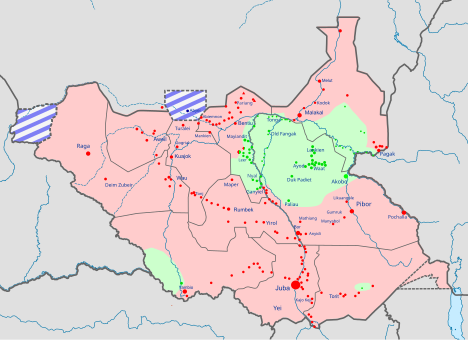
\includegraphics[width=10cm]{figures/Southern_Sudan_Civil_War.svg.png}
  \caption{Military situation in South Sudan on 22 March 2022 \href{https://en.wikipedia.org/wiki/South_Sudanese_Civil_War\#Background}{Wikipedia}}
  \label{fig:label}
\end{figure}

Red - Under control of the Government of South Sudan

Green - Under control of the Sudan People's Liberation Movement-in-Opposition

Blue - Under control of the Government of Sudan

\section{Economic repercussions}
\paragraph{South Sudan} \mbox{}\\
The ongoing violence has significantly impacted oil production in South Sudan, as Chinese and Indian oil workers left when the war began. The oil extraction sector, known as the lifeline of South Sudan, saw a reduction in production that further weakened the state's fragile economy. Consequently, the government struggled to pay salaries for its workers and militias. Priority was given to paying Ugandan forces and those who immediately went to war zones, leaving other staff underpaid \cite{observer2014military}.
\paragraph{Sudan} \mbox{}\\
Sudan's economy suffered from reduction of its revenue from oil after South Sudan's independence. Apart from that, Sudan suffered from currency depreciation, hyperinflation and rise of prices to the basic goods. 

%можно прочесть в https://journals.sagepub.com/doi/epub/10.1177/2233865915573797


\section{Meanwhile in Sudan..}
\subsection{Wave of protests in Sudan}
With hindsight, the September 2013 events were a forerunner of the ongoing wave of popular protests against al-Bashir and his government. The new generation of protestors, mostly students and young professionals, eschewed the hierarchical structures of the established political parties and forged their own horizontal networks supported by the widespread use of the internet. 
\subsection{Bashir arrest warrant}
In 2009, the International Criminal Court issued an arrest warrant for Sudanese President Omar al-Bashir on charges of war crimes and crimes against humanity in Darfur. This warrant highlighted the international community's response to the atrocities committed during the conflict.

\subsection{Fall of Bashir}
In April 2019, after months of protests and civil unrest, Omar al-Bashir was ousted from power in a military coup. His removal marked the end of a 30-year rule and initiated a transitional period aimed at establishing a civilian government.

\newpage
\bibliography{references}
\bibliographystyle{apalike}




\end{document}
